\section{Newsfeed App}
\label{section:newsfeed_app}

\subsection{Beschreibung}

Die native Newsfeed-App ist inspiriert von Twitter. Hier sollen verschiedene News des Unternehmens, des Standorts, in dem der Mitarbeiter arbeitet sowie dessen eigener Abteilung angezeigt werden. In diese Newsfeed-App soll die Umfrage automatisch eingebettet werden, entweder als Banner an der Seite oder als eigener Eintrag im Feed. So können die Mitarbeiter die aktuellen News einsehen und aus eigener Initiative die Umfrage starten.

\subsection{Mockup}

\begin{figure}[H] 
\centering 
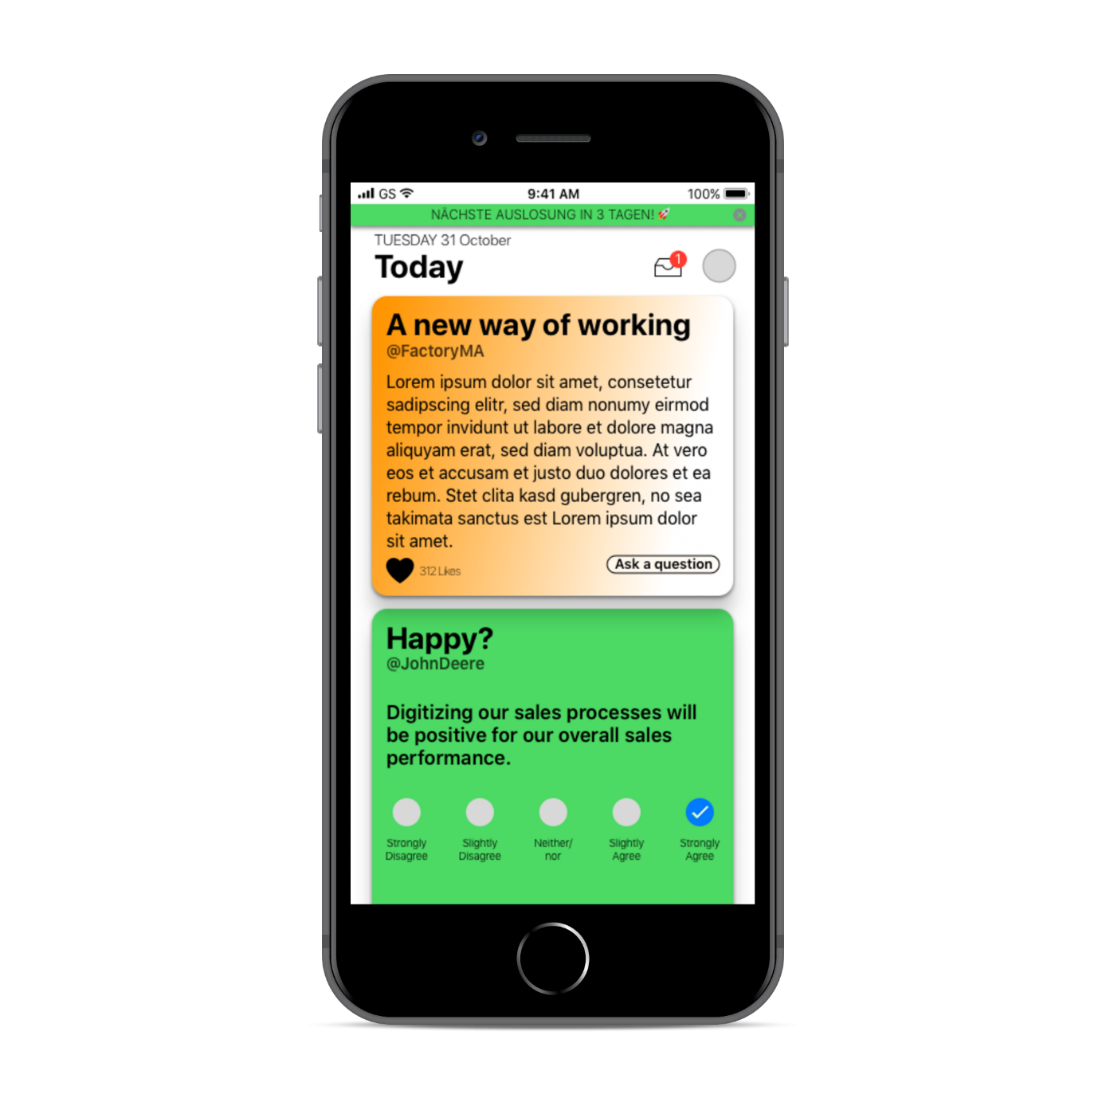
\includegraphics[scale=0.72]{images/5mockup} 
\caption[Mockup: Native Newsfeed-App]{Mockup: Native Newsfeed-App\protect} 
\label{ws} 
\end{figure}

\subsection{Kostenkalkulation}

\subsubsection{Initiale Kosten}

Einmalige Kosten fallen bei der Erstellung der nativen Anwendung an. Diese soll so implementiert werden, dass sie auf allen Endgeräten, insbesondere auf dem Smartphone, genutzt werden kann. Dabei ist es auch hier ein Authentifizierungsmechanismus entscheidend, sodass der Nutzer nur die für ihn bestimmten News erhält.
Schätzung: zwischen 350€ und 1200€.

\subsubsection{Regelmäßige Kosten}

Die native Anwendung muss möglichst jeden Tag bzw. jede Woche um neue News ergänzt werden, sodass der Nutzer auch den Ansporn hat, sie sich anzuschauen. 

\begin{itemize}
\item Abgestellter Mitarbeiter für News für das ganze Unternehmen auf Vollzeit:	2500€ im Monat
\item Abgestellter für News des jeweiligen Standorts je 2 Stunden die Woche:	80€ im Monat
\item Vorarbeiter in der Abteilung je 2 Stunden die Woche:	80€ im Monat
\item Gesamte Kosten:	2660€
\end{itemize}


\subsection{Beurteilung des Projektteams}

\paragraph{Vorteile}

\begin{itemize}
\item	Mitarbeiter erhalten News über das Unternehmen, ggf. bessere Corporate Identity.
\item Die Umfrage ist direkt integriert und somit nicht zu aufdringlich.
\item Die News können die Mitarbeiter anregen, an den Umfragen teilzunehmen, da sie den Inhalt sowohl positiven als auch negativen auffassen können und sich daraufhin dazu äußern wollen.
\end{itemize}

\paragraph{Nachteile}

\begin{itemize}
\item Die Nutzung der Newsfeed App ist fragwürdig, da es wahrscheinlich nur wenige Mitarbeiter gibt, die sich außerhalb der Arbeitszeit damit beschäftigen wollen.
\item Der durchschnittliche Werksmitarbeiter ist womöglich technisch nicht so interessiert, dass er sich eine solche Newsfeed-App herunterladen möchte.
\item Der Kostenaufwand, um die News möglichst aktuell zu halten, ist relativ hoch.
\end{itemize}

\paragraph{Bewertung und Potential}

Die Newsfeed-App wäre gegebenenfalls für technisch interessierte und engagierte Mitarbeiter geeignet. Da dies aber auf einen Großteil der Werksmitarbeiter nicht zutrifft und auch die Möglichkeiten, viele interessante News zu verfassen, relativ gering sind, schätzen wir das Potential einer Newsfeed-App für diesen Use-Case als gering ein. Auch ist der Aufwand, explizit News zu verfassen, unverhältnismäßig groß im Vergleich zu dem, wofür die App eigentlich dienen soll, nämlich dem Anregen, an einer Umfrage teilzunehmen.

\subsection{Feedback und Beurteilung durch PulseShift}

Die Newsfeed App wird  insgesamt von PulseShift positiv bewertet, aber wahrscheinlich vom Kunden kritisch, da diese Content pflegen müssen. Hier gibt es bereits Lösungen von anderen Unternehmen (z.B. MS Staffhub). Es ist sinnvoller, diese zu analysieren und zu evaluieren anstelle eine eigene Anwendung zu entwickeln. 

Folgende Aspekte sollten bei einer Analyse auf jeden Fall berücksichtigt werden: 

\begin{itemize}
\item Flexibilität und Freiraum
\item Anreize zur Nutzung des Bandarbeiters
\item API die durch PulseShift angesprochen werden kann
\item Umfragefunktionalitäten
\item Referenzkunden
\end{itemize}

\subsection{Weiteres Vorgehen}

Es sollen die wichtigsten Lösungen am Markt insbesondere nach den oben genannten Kriterien analysiert und evaluiert werden. Diese Herangehensweise findet in Kapitel 6.3 statt.
